%=======================================================================
%  CS222 - Seminar - Prompting & PEFT - Group 5
%  Master file. Compile with XeLaTeX (twice).
%
%    xelatex -interaction=nonstopmode -halt-on-error main.tex
%    xelatex -interaction=nonstopmode -halt-on-error main.tex
%
%  Overleaf: upload the zip produced by `make zip` and set the compiler to
%  XeLaTeX. Every path here is relative, so the folder compiles as-is.
%=======================================================================
\documentclass[aspectratio=169,10pt]{beamer}

% ---------------------------- Encodings & fonts ------------------------
\usepackage{fontspec}
\usepackage[vietnamese]{babel}

% ---------------------------- Math & symbols ---------------------------
\usepackage{amsmath,amssymb}

% ---------------------------- Text & layout ----------------------------
\usepackage{array}
\usepackage{booktabs}
\usepackage{ragged2e}
\usepackage{graphicx}
\usepackage[dvipsnames,table]{xcolor}
\usepackage{tikz}
\usetikzlibrary{arrows.meta,positioning,fit,backgrounds,calc,shapes.geometric}

% ---------------------------- Links ------------------------------------
\usepackage{hyperref}

% \mathds{1}: the indicator, in the maths font (no dsfont dependency).
\newcommand{\mathds}[1]{\ifmmode\mathbb{#1}\else$\mathbb{#1}$\fi}

\setbeamertemplate{caption}[numbered]
\setbeamertemplate{navigation symbols}{}
\setbeamersize{text margin left=0.55cm, text margin right=0.55cm}
\newlength{\sidemargin}\setlength{\sidemargin}{0.55cm}
\setlength{\leftmargini}{1.1em}
\setlength{\leftmarginii}{1.0em}
\setlength{\parskip}{0.15em}

% ---------------------------- Theme ------------------------------------
\usetheme{default}

\definecolor{Navy}{HTML}{16283F}
\definecolor{NavySoft}{HTML}{2C4A6E}
\definecolor{Amber}{HTML}{E39A1B}
\definecolor{AmberSoft}{HTML}{FFF4DE}
\definecolor{Ink}{HTML}{1B1F24}
\definecolor{Muted}{HTML}{5A6673}
\definecolor{Rule}{HTML}{C9D2DC}
\definecolor{Panel}{HTML}{F3F6F9}
\definecolor{PaperGreen}{HTML}{0E7A4E}

\setbeamercolor{normal text}{fg=Ink}
\setbeamercolor{structure}{fg=Navy}
\setbeamercolor{frametitle}{fg=Navy}
\setbeamercolor{title}{fg=Navy}
\setbeamercolor{alerted text}{fg=Amber!85!black}
\setbeamercolor{block title}{bg=Navy,fg=white}
\setbeamercolor{block body}{bg=Panel,fg=Ink}
\setbeamercolor{block title alerted}{bg=Amber!90!black,fg=white}
\setbeamercolor{block body alerted}{bg=AmberSoft,fg=Ink}
\setbeamercolor{itemize item}{fg=Navy}
\setbeamercolor{itemize subitem}{fg=NavySoft}
\setbeamercolor{caption name}{fg=Muted}
\setbeamercolor{page number in head/foot}{fg=Muted}

\setbeamerfont{normal text}{size=\small}
\setbeamerfont{frametitle}{size=\normalsize,series=\bfseries}
\setbeamerfont{title}{size=\LARGE,series=\bfseries}
\setbeamerfont{subtitle}{size=\large}
\setbeamerfont{block title}{size=\small,series=\bfseries}
\setbeamerfont{block body}{size=\small}
\setbeamerfont{itemize/enumerate body}{size=\small}
\setbeamerfont{caption}{size=\scriptsize}
\setbeamerfont{footline}{size=\scriptsize}

\setbeamertemplate{itemize item}{\usebeamercolor[fg]{itemize item}\scriptsize\hbox to 1.25em{$\blacktriangleright$\hfil}}
\setbeamertemplate{itemize subitem}{\usebeamercolor[fg]{itemize subitem}\scriptsize\hbox to 1.1em{$\bullet$\hfil}}
\setbeamertemplate{enumerate item}{\color{Navy}\insertenumlabel.}

% ---------------------------- Frame title with accent rule -------------
\setbeamertemplate{frametitle}{%
  \vspace*{0.30em}%
  {\usebeamercolor[fg]{frametitle}\usebeamerfont{frametitle}\insertframetitle}%
  \ifx\insertframesubtitle\empty\else
    \hspace{0.55em}{\normalfont\small\color{Muted}\insertframesubtitle}%
  \fi
  \par\nobreak\vspace{0.18em}%
  \noindent{\color{Amber}\rule{\textwidth}{1.1pt}}%
  \par\vspace{0.10em}%
}

% ---------------------------- Footer -----------------------------------
\setbeamertemplate{footline}{%
  \leavevmode%
  \hbox{%
    \begin{beamercolorbox}[wd=.325\paperwidth,ht=2.2ex,dp=1.1ex,left]{page number in head/foot}%
      \hspace*{\sidemargin}Nhóm 5 --- UIT%
    \end{beamercolorbox}%
    \begin{beamercolorbox}[wd=.345\paperwidth,ht=2.2ex,dp=1.1ex,center]{page number in head/foot}%
      CS222 --- Prompting \& PEFT%
    \end{beamercolorbox}%
    \begin{beamercolorbox}[wd=.33\paperwidth,ht=2.2ex,dp=1.1ex,right]{page number in head/foot}%
      \insertframenumber{}\,/\,\inserttotalframenumber\hspace*{\sidemargin}%
    \end{beamercolorbox}}%
  \vspace*{0.2ex}%
}

% ---------------------------- Helper commands --------------------------
\newcommand{\tightlist}{%
  \setlength{\itemsep}{0.3em}%
  \setlength{\parskip}{0.1em}%
}

% A figure scaled to the available width, never taller than #1 text-heights.
\newcommand{\FigureFull}[3][0.62]{%
  \begin{center}
    \includegraphics[width=\linewidth,height=#1\textheight,keepaspectratio]{figure/#2}%
    \par\vspace{0.25em}{\color{Muted}\scriptsize #3}%
  \end{center}%
}

% One-line conclusion, anchored under the content of a frame.
\newcommand{\Takeaway}[1]{%
  \par\vspace{0.3em}%
  \noindent\begin{beamercolorbox}[wd=\dimexpr\linewidth-1em\relax,sep=0.45em]{block title alerted}
    \raggedright\footnotesize\emergencystretch=1.5em \textbf{Điểm chốt.}~#1
  \end{beamercolorbox}%
}

% A question the speakers pose to the room.
\newcommand{\Ask}[1]{%
  \par\vspace{0.3em}%
  \noindent\begin{beamercolorbox}[wd=\dimexpr\linewidth-1em\relax,sep=0.45em]{block body alerted}
    \raggedright\footnotesize\textbf{\color{Amber!70!black}Câu hỏi.}~#1
  \end{beamercolorbox}%
}

% Small titled card, three per row on the task-type slides.
\newcommand{\TaskCard}[2]{%
  \begin{minipage}[t]{0.32\linewidth}
    \begin{beamercolorbox}[wd=\linewidth,sep=0.45em]{block body}
      \footnotesize\raggedright\textbf{#1}\par\vspace{0.15em}
      {\scriptsize\color{Muted}#2}
    \end{beamercolorbox}
  \end{minipage}}

% Table cell helpers: green = beats the oracle / multi-task baseline,
% bold = the best in the column.
\newcommand{\Best}[1]{\textbf{#1}}
\newcommand{\Win}[1]{{\color{PaperGreen}\textbf{#1}}}
\newcommand{\Dim}[1]{{\color{Muted}#1}}
\newcommand{\cell}[1]{\ensuremath{#1}}

% ---------------------------- Metadata ---------------------------------
\title[CS222 --- Prompting \& PEFT]{Prompting \& PEFT: Phần ứng dụng}
\subtitle{GEPA --- Reflective Prompt Evolution \quad$\cdot$\quad Text-to-LoRA --- Instant Transformer Adaptation}
\author[Nhóm 5 --- UIT]{%
  Nhóm 5: \textbf{Bùi Huỳnh Tây} \and \textbf{Lê Thiên Quân} \and \textbf{Đoàn Hồng Bảo}%
}
\institute[UIT]{%
  GVHD: TS. Nguyễn Thị Quý\\
  Trường Đại học Công nghệ Thông tin --- ĐHQG TP.HCM
}
\date[Xử lý ngôn ngữ tự nhiên nâng cao]{Xử lý ngôn ngữ tự nhiên nâng cao --- CS222}

\begin{document}

% ------------------------------------------------------------------ 1
\begin{frame}[plain]
  \begin{tikzpicture}[remember picture, overlay]
    \fill[Navy] (current page.north west) rectangle ([yshift=-0.62\paperheight]current page.north east);
    \fill[Amber] ([yshift=-0.62\paperheight]current page.north west) rectangle ([yshift=-0.628\paperheight]current page.north east);
    \node[anchor=north west, text=white!88, align=left, font=\scriptsize]
      at ([xshift=0.7cm, yshift=-0.45cm]current page.north west) {%
      ĐẠI HỌC QUỐC GIA TP. HỒ CHÍ MINH\\[0.1em]
      TRƯỜNG ĐẠI HỌC CÔNG NGHỆ THÔNG TIN};
    \node[anchor=west, text=white, align=left, font=\LARGE\bfseries, text width=13.4cm]
      at ([xshift=0.7cm, yshift=0.9cm]current page.west) {%
      PROMPTING \& PEFT\\[0.15em] PHẦN ỨNG DỤNG};
    \node[anchor=south west, text=white!92, align=left, font=\footnotesize]
      at ([xshift=0.7cm, yshift=0.35cm]current page.south west) {%
      Xử lý ngôn ngữ tự nhiên Nâng cao};
  \end{tikzpicture}

  \vspace{0.48\textheight}
  \begin{columns}[T,onlytextwidth]
    \begin{column}{0.52\textwidth}
      {\color{Muted}\scriptsize GVHD}\\[0.15em]
      {\bfseries TS. Nguyễn Thị Quý}\\[0.9em]
      {\color{Muted}\scriptsize Nhóm 5}\\[0.15em]
      {\bfseries Bùi Huỳnh Tây \,--\, Lê Thiên Quân \,--\, Đoàn Hồng Bảo}
    \end{column}
    \begin{column}{0.44\textwidth}
      \raggedleft
      {\color{Muted}\scriptsize Học phần}\\[0.15em]
      {\bfseries Xử lý ngôn ngữ tự nhiên Nâng cao}
    \end{column}
  \end{columns}
\end{frame}

% ------------------------------------------------------------------ 2
\begin{frame}{Nội dung}
  \begin{enumerate}\tightlist
    \item Bài toán Downstream Task
    \item Prompting: GEPA --- ICLR 2026
    \item PEFT: Text-to-Lora --- ICML 2025
    \item Quy trình Thực nghiệm \& Kết hợp 2 phương pháp.
  \end{enumerate}
\end{frame}


%=======================================================================
%  Slides 3-15 - Bài toán Downstream Task
%   Transcribed 1:1 from slide-cs222.pptx.pdf (same order, same wording).
%=======================================================================
\section{Bài toán Downstream Task}

% ------------------------------------------------------------------ 3
\begin{frame}{Nội dung chương 1}
  \begin{columns}[T,onlytextwidth]
    \begin{column}{0.5\textwidth}
      \begin{enumerate}\tightlist
        \item[\textbf{1.1}] Giới thiệu bài toán
        \item[\textbf{1.2}] Phương pháp
        \item[\textbf{1.3}] Hạn chế
      \end{enumerate}
    \end{column}
    \begin{column}{0.44\textwidth}
      \begin{beamercolorbox}[wd=\dimexpr\linewidth-1em\relax,sep=0.6em]{block body}
        \footnotesize\color{Muted}
        \centering 1. Bài toán Downstream Task
      \end{beamercolorbox}
    \end{column}
  \end{columns}
\end{frame}

% ------------------------------------------------------------------ 4
\begin{frame}{1.1\quad Giới thiệu bài toán}
  \begin{columns}[T,onlytextwidth]
    \begin{column}{0.53\textwidth}
      \justifying
      Model là một mô hình ngôn ngữ đã qua ký hiệu là $M$, sở hữu bộ trọng số gốc
      $\theta_0$.

      \vspace{0.35em}
      Đầu ra của model $M$ trên 1 đầu vào $x$ bị ảnh hưởng bởi 2 thành phần:
      \begin{itemize}\tightlist
        \item $\pi$: Prompt (chỉ dẫn hay ngữ cảnh ở không gian đầu vào)
        \item denta\_$\theta$: Phần cập nhật trọng số.
      \end{itemize}
    \end{column}
    \begin{column}{0.43\textwidth}
      \begin{beamercolorbox}[wd=\dimexpr\linewidth-1em\relax,sep=0.7em]{block body}
        \centering\footnotesize
        Đầu ra của model $M$ với input $x$:\\[0.4em]
        {\large $y = M(x;\ \pi,\ \theta_0 + \Delta\theta)$}
      \end{beamercolorbox}
    \end{column}
  \end{columns}
\end{frame}

% ------------------------------------------------------------------ 5
\begin{frame}{1.1\quad Giới thiệu bài toán}
  \justifying
  \textbf{Downsteam Task Adaptation} là quá trình điều chỉnh một Model ($M$) để nó
  giải quyết tốt một bài toán cụ thể ($T$), thay vì phải huấn luyện một mô hình mới
  từ đầu.

  \vspace{0.3em}
  Đặt $D_T$ là tập phân phối dữ liệu $(x, m)$ của task $T$.
  \begin{itemize}\tightlist
    \item Với $x$ là input của task $T$.
    \item Với $m$ là đáp án đúng của task $T$.
  \end{itemize}

  \begin{beamercolorbox}[wd=\dimexpr\linewidth-1em\relax,sep=0.5em]{block body}
    \centering\footnotesize
    Nhiệm vụ:\\[0.3em]
    $(\pi^*, \Delta\theta^*) = \arg\max_{(\pi, \Delta\theta)}\ \mathbb{E}_{((x,\,m)\sim D_T)}\big[\ \mu(M(x;\ \pi,\ \theta_0 + \Delta\theta),\ m)\ \big]$
  \end{beamercolorbox}
  \vspace{0.2em}
  $\Leftrightarrow$ \textbf{Mục tiêu:} tìm bộ trọng số $\theta^*$ và bộ prompt $\pi^*$ tốt nhất.
\end{frame}

% ------------------------------------------------------------------ 6
\begin{frame}{1.1\quad Giới thiệu bài toán}
  Ví dụ một số downstream task:
  \begin{itemize}\tightlist
    \item Suy luận giải Toán
    \item Hỏi đáp suy luận đa bước
    \item Kiểm chứng thông tin
    \item Tuân thủ hướng dẫn phức tạp
    \item Tối ưu hoá mã nguồn
    \item \dots
  \end{itemize}
\end{frame}

% ------------------------------------------------------------------ 7
\begin{frame}{1.1\quad Giới thiệu bài toán: Downstream Task}
\end{frame}

% ------------------------------------------------------------------ 8
\begin{frame}{1.1\quad Giới thiệu bài toán}
  \FigureFull[0.66]{t2l/fig4_qualitative}{Hình 4 --- Text-to-LoRA (ICML 2025)}
\end{frame}

% ------------------------------------------------------------------ 9
\begin{frame}{1.2\quad Phương pháp cho DTA}
  \textbf{Hướng tối ưu prompt ($\pi$)}
  \begin{itemize}\tightlist
    \item In-Context Learning:
      \begin{itemize}\tightlist
        \item Few-shot
        \item Chain of Thought
        \item Self-Consistency
        \item Tree-of-Thoughts
        \item \dots
      \end{itemize}
  \end{itemize}
\end{frame}

% ------------------------------------------------------------------ 10
\begin{frame}{1.2\quad Phương pháp cho DTA}
  \textbf{Hướng tối ưu prompt:}
  \begin{itemize}\tightlist
    \item In-Context Learning:
    \item Automated Optimization:
      \begin{itemize}\tightlist
        \item LLM-as-an-Optimizer: Dùng LLM để tối ưu prompt
        \item EvoPrompt: Dùng thuật toán tiến hoá.
        \item RL-based Prompting: Dùng RL huấn luyện một mô hình nhỏ để sinh ra chuỗi
              token prompt giúp tối đa hóa phần thưởng.
        \item Hệ thống có nhiều LLM (Compound AI System):
          \begin{itemize}\tightlist
            \item Tối ưu đồng bộ cả câu chỉ dẫn lẫn bộ mẫu few-shot cho toàn bộ
                  pipeline gồm nhiều module LLM nối tiếp nhau. (DSPy, MIPROv2).
          \end{itemize}
      \end{itemize}
  \end{itemize}
\end{frame}

% ------------------------------------------------------------------ 11
\begin{frame}{1.2\quad Phương pháp cho DTA}
  \textbf{Hướng tối ưu tham số mô hình ($\theta$)}
  \begin{itemize}\tightlist
    \item Full Fine-Tuning (FFT)
    \item Parameter-Efficient Fine-Tuning (PEFT): Đóng băng gần như toàn bộ mô hình gốc,
          chỉ huấn luyện số lượng tham số $\ll$ tổng số tham số.
      \begin{itemize}\tightlist
        \item Reparameterization: LoRa, QLoRa, \dots
        \item Adapters
        \item Prefix-Tuning / Prompt-Tuning
      \end{itemize}
  \end{itemize}
\end{frame}

% ------------------------------------------------------------------ 12
\begin{frame}{1.3\quad Hạn chế của từng phương pháp}{Hạn chế của hướng Prompt}
  \begin{itemize}\tightlist
    \item In Context Learning thủ công:
      \begin{itemize}\tightlist
        \item Phụ thuộc vào kinh nghiệm thử-sai, cách diễn đạt câu chữ và thứ tự sắp
              xếp ví dụ.
        \item Không biết đưa ví dụ few-shot nào phù hợp.
        \item Hệ thống gồm nhiều LLMs (Compound AI System) thì sẽ rất khó để chỉnh tay
              tất cả.
      \end{itemize}
  \end{itemize}
  \vspace{0.3em}
  $\rightarrow$ Automated Optimization ra đời.
\end{frame}

% ------------------------------------------------------------------ 13
\begin{frame}{1.3\quad Hạn chế của từng phương pháp}{Hạn chế của Automated Optimization Prompt}
  \begin{itemize}\tightlist
    \item Tốn nhiều lượt chạy (Rollout) mới tìm được prompt tốt.\\
          $\rightarrow$ Chi phí về Rollout Budget
    \item Prompt bị phình to (Các pp sẽ overfit bằng cách gom nhiều ví dụ few-shot vào
          để tăng điểm)\\
          $\rightarrow$ Chi phí về Inference Token Budget.
  \end{itemize}
  \vspace{0.4em}
  Phương pháp GEPA sẽ giải quyết 2 vấn đề trên.
\end{frame}

% ------------------------------------------------------------------ 14
\begin{frame}{1.3\quad Hạn chế của từng phương pháp}{Hạn chế của PEFT}
  \begin{itemize}\tightlist
    \item Dù PEFT đã cắt giảm mạnh chi phí VRAM so với Full Fine-Tuning và giữ được chi
          phí suy luận thấp nhưng:
      \begin{itemize}\tightlist
        \item Chi phí thích nghi lặp lại theo từng tác vụ: Bản chất của PEFT truyền
              thống vẫn là huấn luyện chuyên biệt cho từng bài toán.
        \item Zero-shot Adaption: Khác với Prompting có thể chuyển sang tác vụ mới ngay
              lập tức chỉ bằng vài dòng mô tả, PEFT không thể phản ứng tức thời khi chưa
              có dữ liệu và thời gian train.
      \end{itemize}
  \end{itemize}
\end{frame}

% ------------------------------------------------------------------ 15
\begin{frame}{1.3\quad Hạn chế của từng phương pháp}
  \justifying
  Làm sao để giữ được ưu thế cập nhật trọng số và tốc độ suy luận của LoRA, nhưng xóa bỏ
  hoàn toàn chi phí dữ liệu và thời gian huấn luyện lại mỗi khi gặp tác vụ mới?

  \vspace{0.6em}
  \begin{beamercolorbox}[wd=\dimexpr\linewidth-1em\relax,sep=0.6em]{block title alerted}
    $\rightarrow$ Text-to-LoRA giải quyết nút thắt này bằng kiến trúc Hypernetwork, cho
    phép sinh trực tiếp ma trận trọng số LoRA ngay từ văn bản mô tả tác vụ chỉ trong
    1 lượt chạy xuôi.
  \end{beamercolorbox}
\end{frame}

%=======================================================================
%  Slides 16-41 - Prompting: GEPA (ICLR 2026)
%=======================================================================
\section{Prompting: GEPA}

% ------------------------------------------------------------------ 16
\SectionSlide{2. GEPA}{Reflective Prompt Evolution Can Outperform RL}{%
  \small
  \begin{tabular}{@{}l@{\hspace{0.6em}}l@{}}
    \textbf{2.1} & \textbf{Bài toán}\\
    \textbf{2.2} & \textbf{Một số công trình liên quan}\\
                 & {\color{white!80}2.2.1 Prompt Opt (MIPROv2)}\\
                 & {\color{white!80}2.2.2 EvoPrompt}\\
    \textbf{2.3} & \textbf{Pipeline GEPA}\\
                 & {\color{white!80}2.3.1 Chọn lọc trên biên Pareto}\\
                 & {\color{white!80}2.3.2 Đột biến bằng Phản chiếu}\\
                 & {\color{white!80}2.3.3 System-aware Merge}\\
    \textbf{2.4} & \textbf{Kết quả thực nghiệm}\\
    \textbf{2.5} & \textbf{Giới hạn \& Tổng kết}
  \end{tabular}}

% ------------------------------------------------------------------ 17
\begin{frame}{2.1\quad Bài toán}
  \vspace{0.4em}
  \centering\DeckFig[0.78]{compound_ai}{0.88\linewidth}
\end{frame}

% ------------------------------------------------------------------ 18
\begin{frame}{2.1\quad Bài toán}
  \begin{itemize}\setlength{\itemsep}{0.8em}
    \item Hệ thống gồm $\mathbf{k}$ module LLM nối tiếp nhau.
    \item Mỗi module $i$ được điều khiển bởi prompt $\pi_i$
    \item Một ứng viên hệ thống là tập prompt: $\Phi = \{\pi_1, \pi_2, \dots, \pi_k\}$
    \item Toàn bộ trọng số mô hình gốc ($\theta$) được đóng băng $\rightarrow$ chỉ tối ưu
          trên không gian văn bản rời rạc
  \end{itemize}
\end{frame}

% ------------------------------------------------------------------ 19
\begin{frame}{2.2\quad Một số công trình liên quan}
  \Sub{2.2.1 MIPROv2 --- {\normalfont\href{https://arxiv.org/abs/2406.11695}{\color{NavySoft}\underline{https://arxiv.org/abs/2406.11695}}}}
  \vspace{0.4em}
  \begin{itemize}\setlength{\itemsep}{0.6em}
    \item \textbf{Chuẩn mực SOTA \& đối thủ so sánh trực tiếp} của GEPA trong nhánh tối ưu
          Prompt tự động (Bayesian Optimization) cho hệ thống nhiều bước (Compound AI System)
    \item Đóng băng trọng số mô hình gốc ($\theta$), chỉ tìm tổ hợp bộ chỉ dẫn (instruction)
          và ví dụ mẫu (few-shot) tối ưu
  \end{itemize}
\end{frame}

% ------------------------------------------------------------------ 20
\begin{frame}{2.2\quad Một số công trình liên quan}
  \begin{columns}[T,onlytextwidth]
    \begin{column}{0.66\textwidth}
      \Sub{2.2.1 MIPROv2 --- Cơ chế hoạt động:}
      \begin{enumerate}\setlength{\itemsep}{0.5em}
        \item \textbf{Bootstrapping:} Chạy hệ thống trên dữ liệu mẫu để thu thập các cặp ví
              dụ few-shot thành công
        \item \textbf{Grounded Proposal:} Dùng LLM sinh ra nhiều ứng viên câu chỉ dẫn dựa
              trên mô tả tác vụ và dữ liệu
        \item \textbf{Tìm kiếm tổ hợp} (Bayesian Optimization): Đánh giá trên tập validation
              để chọn tổ hợp (Instruction $+$ Few-shot) tốt nhất cho từng module
      \end{enumerate}
    \end{column}
    \begin{column}{0.31\textwidth}
      \centering\vspace{-0.3em}\DeckFig[0.74]{miprov2}{\linewidth}
    \end{column}
  \end{columns}
\end{frame}

% ------------------------------------------------------------------ 21
\begin{frame}{2.2\quad Một số công trình liên quan}
  \Sub{2.2.1 MIPROv2 --- Hạn chế:}
  \vspace{0.3em}
  \begin{itemize}\setlength{\itemsep}{0.7em}
    \item Vẫn dựa chủ yếu vào điểm số tổng (scalar metric)\\
          $\rightarrow$ bỏ phí thông tin chẩn đoán từ dấu vết lỗi sai (execution traces)
    \item Có xu hướng nhồi nhiều ví dụ few-shot để kéo điểm\\
          $\rightarrow$ prompt sinh ra rất dài, làm đội Inference Token Budget và tăng độ
          trễ suy luận
  \end{itemize}
\end{frame}

% ------------------------------------------------------------------ 22
\begin{frame}{2.2\quad Một số công trình liên quan}
  \Sub{2.2.2 EvoPrompt --- {\normalfont\href{https://arxiv.org/abs/2309.08532}{\color{NavySoft}\underline{https://arxiv.org/abs/2309.08532}}}}
  \vspace{0.4em}
  \begin{itemize}\setlength{\itemsep}{0.6em}
    \item \textbf{Tiền đề (Motivation)} cho khung tiến hóa của GEPA: kết hợp
          \textbf{Thuật toán tiến hóa} với LLM để tối ưu prompt tự động
    \item Duy trì một quần thể nhiều prompt ứng viên qua các thế hệ
    \item Ở mỗi vòng lặp: chọn các prompt có điểm đánh giá cao, dùng LLM thực hiện
          \textbf{Đột biến} và \textbf{Lai ghép} để sinh prompt mới
  \end{itemize}
\end{frame}

% ------------------------------------------------------------------ 23
\begin{frame}{2.2\quad Một số công trình liên quan}
  \Sub{2.2.2 EvoPrompt --- Hạn chế:}
  \vspace{0.3em}
  \begin{itemize}\setlength{\itemsep}{0.65em}
    \item \textbf{Đột biến ``mù quáng'':} Chỉ sửa câu chữ ngẫu nhiên dựa trên điểm số, không
          biết prompt sai ở bước nào $\rightarrow$ thử sai tốn kém, hội tụ chậm
    \item \textbf{Chọn lọc theo điểm trung bình:} Dễ làm mất sự đa dạng và bị kẹt ở cực trị
          địa phương
    \item \textbf{Chỉ tối ưu 1 prompt đơn lẻ:} Khó mở rộng sang hệ thống nhiều prompt (module)
          nối tiếp nhau (\textbf{Compound AI System})
  \end{itemize}
  \vspace{0.4em}
  \begin{beamercolorbox}[wd=\linewidth,sep=0.55em]{block body}
    $\Rightarrow$ \textbf{Động lực của GEPA:} Giữ khung tiến hóa nhưng nâng cấp bằng
    \textbf{Đột biến Phản chiếu}, \textbf{Biên Pareto} và \textbf{Lai ghép theo cấu trúc (LCA)}.
  \end{beamercolorbox}
\end{frame}

% ------------------------------------------------------------------ 24
\begin{frame}{2.3\quad GEPA}
  \Sub{Thiết lập dữ liệu}
  \begin{itemize}\setlength{\itemsep}{0.45em}
    \item \textbf{Chia tập $D_{\text{train}}$ thành 2 phần tách biệt}:
      \begin{itemize}\tightlist
        \item $D_{\text{feedback}}$ \textit{(như tập Train)}: Nguồn bốc mẫu cho phần đột biến
              prompt soi lỗi và sửa prompt.
        \item $D_{\text{pareto}}$ \textit{(như Validation nội bộ)}: Tập cố định (vài chục đến
              $\sim$100 mẫu), dùng để chấm điểm như tập validation.
      \end{itemize}
    \item \textbf{Minibatch ($\mathcal{M}$):} Nhóm nhỏ cố định ($b \approx 3$--$5$ mẫu) bốc ngẫu
          nhiên từ $D_{\text{feedback}}$ mỗi vòng $\rightarrow$ vừa đủ ngắn để đọc kỹ lỗi,
          vừa làm vòng loại nhanh.
  \end{itemize}
\end{frame}

% ------------------------------------------------------------------ 25
\begin{frame}{2.3\quad GEPA}
  \Sub{Khái niệm cốt lõi}
  \begin{itemize}\setlength{\itemsep}{0.4em}
    \item \textbf{Prompt khởi tạo ($P_0$):} Bộ prompt cơ bản ban đầu cho $k$ module (viết tay
          ngắn gọn hoặc prompt zero-shot mặc định của framework). \textbf{Không} cần tối ưu
          sẵn --- chỉ cần đúng định dạng để hệ thống chạy được và sinh traces.
    \item \textbf{Candidate Pool ($\mathcal{P}$):} Kho lưu trữ dạng \textbf{cây tiến hóa}
          (gốc là $P_0$), lưu mọi ứng viên vượt qua vòng lọc minibatch kèm bảng điểm trên
          $D_{\text{pareto}}$ và quan hệ cha--con (phục vụ lọc Pareto \& Merge).
    \item \textbf{Rollout:} 1 lượt chạy hoàn chỉnh hệ thống AI trên 1 mẫu dữ liệu.
    \item \textbf{Rollout Budget ($B$):} Siêu tham số giới hạn tổng số lượt Rollout tối đa
          (\texttt{While Budget > 0}); hết ngân sách thì dừng và chọn ứng viên điểm trung bình
          cao nhất trên $D_{\text{pareto}}$.
  \end{itemize}
\end{frame}

% ------------------------------------------------------------------ 26
\begin{frame}{2.3\quad GEPA}
  \centering\DeckFig[0.9]{gepa_flow_vi}{\linewidth}
\end{frame}

% ------------------------------------------------------------------ 27
\begin{frame}{2.3\quad GEPA}
  \centering
  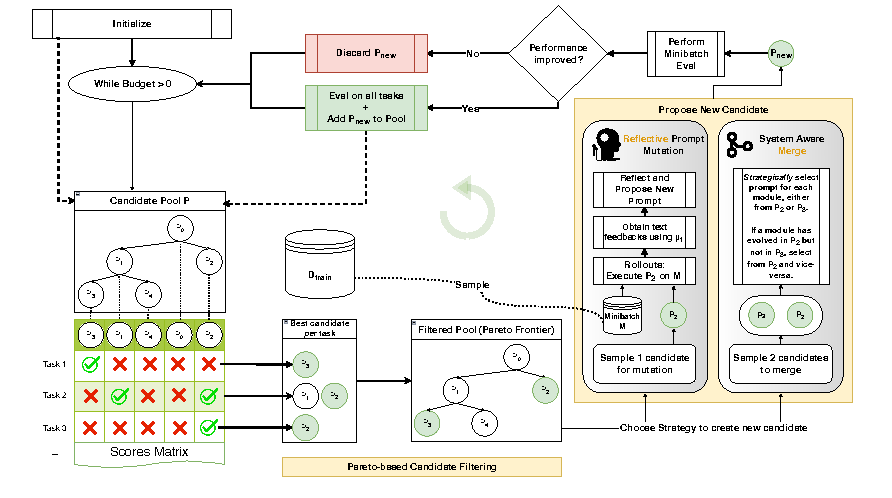
\includegraphics[width=\linewidth,height=0.9\textheight,keepaspectratio]{figure/gepa/fig3_pipeline}
\end{frame}

% ------------------------------------------------------------------ 28
\begin{frame}{2.3\quad GEPA}
  \Sub{2.3.1 Thuật toán: Chọn lọc trên biên Pareto}
  \begin{itemize}\setlength{\itemsep}{0.35em}
    \item Chỉ giữ 1 ứng viên có điểm trung bình cao nhất\\
          $\rightarrow$ dễ mất đa dạng chiến lược và kẹt ở cực trị địa phương
    \item Với mỗi mẫu dữ liệu $x_j \in D_{\text{pareto}}$, tìm điểm số cao nhất mà quần
          thể $\mathcal{P}$ đạt được:
          \[ s^*(x_j) = \max_{\Phi\in\mathcal{P}} s(\Phi, x_j) \]
    \item Chỉ giữ lại các ứng viên đạt đỉnh $s^*(x_j)$ trên ít nhất một mẫu $x_j$ (loại
          bỏ ứng viên bị thống trị hoàn toàn --- dominated)
    \item Xác suất chọn ứng viên $\Phi$: Tỷ lệ thuận với số lượng mẫu $x_j$ mà $\Phi$ đạt
          điểm cao nhất
  \end{itemize}
\end{frame}

% ------------------------------------------------------------------ 29
\begin{frame}{2.3\quad GEPA}
  \Sub{2.3.1 Thuật toán: Chọn lọc trên biên Pareto}
  \centering\DeckFig[0.64]{pareto_filter}{0.92\linewidth}
\end{frame}

% ------------------------------------------------------------------ 30
\begin{frame}{2.3\quad GEPA}
  \begin{columns}[T,onlytextwidth]
    \begin{column}{0.5\textwidth}
      \Sub{2.3.1 Chọn lọc trên biên Pareto}
      \vspace{0.4em}
      \textbf{Ý nghĩa:}
      \begin{itemize}\setlength{\itemsep}{0.6em}
        \item Giữ lại đồng thời các ``chuyên gia'' giải tốt những dạng bài con khác nhau
        \item Cân bằng giữa \textbf{khai thác} (ứng viên giỏi nhiều mẫu) và \textbf{khám
              phá} (ứng viên giỏi các ca khó/ngách)
      \end{itemize}
    \end{column}
    \begin{column}{0.47\textwidth}
      \centering\DeckFig[0.74]{algo2_pareto}{\linewidth}
    \end{column}
  \end{columns}
\end{frame}

% ------------------------------------------------------------------ 31
\begin{frame}{2.3\quad GEPA}
  \Sub{2.3.2 Reflective Prompt Mutation}
  \vspace{0.6em}
  \begin{beamercolorbox}[wd=\linewidth,sep=0.7em]{block body}
    \textbf{Mục tiêu:} Sửa lỗi có chủ đích cho từng module dựa trên dấu vết thực thi
    (thay vì sửa ngẫu nhiên như EvoPrompt).
  \end{beamercolorbox}
\end{frame}

% ------------------------------------------------------------------ 32
\begin{frame}{2.3\quad GEPA}
  \Sub{2.3.2 Reflective Prompt Mutation}
  \begin{itemize}\setlength{\itemsep}{0.3em}
    \item \textbf{Chọn module ($\pi_i$):} Chọn 1 module trong ứng viên $\Phi$ (xoay vòng
          Round-Robin)
    \item \textbf{Chạy thử:} Chạy $\Phi$ trên minibatch $\mathcal{M}$ $\rightarrow$ thu thập
          Execution Traces và phản hồi lỗi ($f$) qua hàm $\mu_f$
    \item \textbf{Phản chiếu (Reflection LM):} Dùng LLM thông thường qua Meta-Prompt đọc
          ($\pi_i$ cũ $+$ Traces $+$ Feedback $f$) $\rightarrow$ chẩn đoán nguyên nhân và viết
          lại $\pi_i$ mới cô đọng, có quy tắc rõ ràng
    \item \textbf{Màng lọc Eval 2 tầng:} Chạy thử $\Phi_{\text{new}}$ trên chính minibatch
          $\mathcal{M}$:
      \begin{itemize}\tightlist
        \item Điểm KHÔNG tăng $\rightarrow$ \textbf{Discard} ngay để tiết kiệm Rollout Budget.
        \item Điểm TĂNG $\rightarrow$ Chấm \textbf{Eval on all tasks} ($D_{\text{pareto}}$)
              và thêm vào quần thể $\mathcal{P}$.
      \end{itemize}
  \end{itemize}
\end{frame}

% ------------------------------------------------------------------ 33
\begin{frame}{2.3\quad GEPA}
  \Sub{2.3.3 System-aware Merge (LCA)}
  \begin{itemize}\setlength{\itemsep}{0.45em}
    \item \textbf{Khi nào kích hoạt?} Sau khi một vòng Đột biến thành công (giới hạn mặc định
          \texttt{max\_merge = 5}), nếu trên Biên Pareto có $\ge 2$ ứng viên thuộc các nhánh
          khác nhau chưa từng ghép
    \item \textbf{Cơ chế ghép theo Tổ tiên chung gần nhất (LCA):}
      \begin{itemize}\tightlist
        \item So sánh từng module của 2 nhánh ($P_A, P_B$) với bản gốc chung $P_{\text{LCA}}$.
        \item Nhánh nào đã nâng cấp module $i$ thì lấy module đó; nếu cả 2 cùng sửa 1 module
              $\rightarrow$ ưu tiên nhánh có điểm tổng cao hơn.
      \end{itemize}
    \item \textbf{Kiểm tra nhanh:} Không tốn lệnh gọi Reflection LM; chạy thử bản ghép
          $P_{\text{merge}}$ trên minibatch $\rightarrow$ nếu không tụt điểm so với $P_A, P_B$
          thì chấm trên $D_{\text{pareto}}$ và thêm vào Pool
  \end{itemize}
\end{frame}

% ------------------------------------------------------------------ 34
\begin{frame}{2.3\quad GEPA}
  \Sub{2.3.3 System-aware Merge}
  \centering
  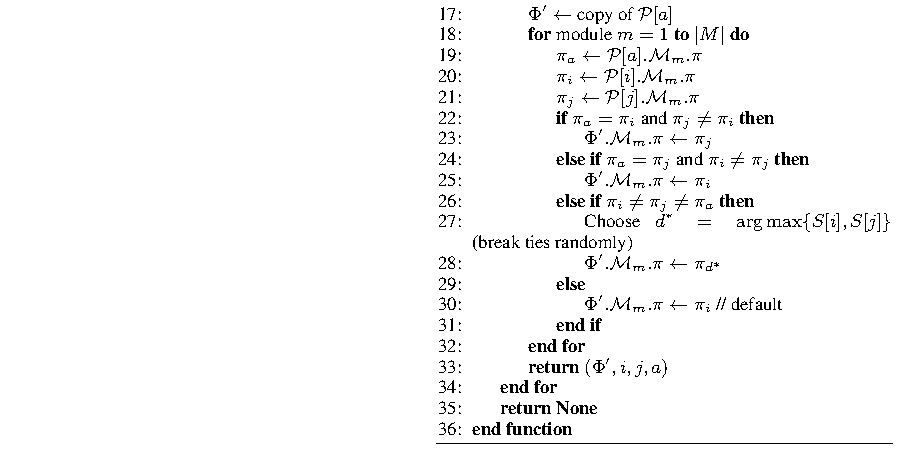
\includegraphics[width=\linewidth,height=0.6\textheight,keepaspectratio]{figure/gepa/fig9_merge}
  \par\vspace{0.2em}{\color{Muted}\scriptsize Hình 9 --- GEPA (ICLR 2026)}
\end{frame}

%=======================================================================
%  Slides 35-39 - 2.4 Kết quả thực nghiệm (Experiments)
%=======================================================================

% ------------------------------------------------------------------ 35
\begin{frame}{2.4\quad Kết quả thực nghiệm}
  \Sub{Thiết lập thực nghiệm (Experimental Setup)}
  \begin{itemize}\setlength{\itemsep}{0.55em}
    \item \textbf{Mô hình đánh giá (2 nhóm):}
      \begin{itemize}\tightlist
        \item Mã nguồn mở: \textbf{Qwen3 8B} (cho phép chạy cả RL và Prompt Opt).
        \item Đóng (Proprietary API): \textbf{GPT-4.1 mini}.
      \end{itemize}
    \item \textbf{4 Benchmark cho Compound AI System:}
      \begin{itemize}\tightlist
        \item \textbf{HotpotQA:} Hỏi--đáp đa bước (multi-hop QA).
        \item \textbf{IFBench:} Tuân thủ chỉ dẫn phức tạp (instruction following).
        \item \textbf{HoVer:} Kiểm chứng thông tin đa bước (fact verification).
        \item \textbf{PUPA:} Ủy quyền bảo mật quyền riêng tư (privacy-preserving delegation).
      \end{itemize}
    \item \textbf{Đối thủ so sánh (Baselines):} Baseline gốc ($P_0$), \textbf{GRPO} (RL SOTA
          trên Qwen3 8B), \textbf{MIPROv2} (Prompt Opt SOTA), và 2 cấu hình \textbf{GEPA} /
          \textbf{GEPA+Merge}.
  \end{itemize}
\end{frame}

% ------------------------------------------------------------------ 36
\begin{frame}{2.4\quad Kết quả thực nghiệm}
  \Sub{Observation 1: Vượt trội GRPO (RL) với số Rollout ít hơn tới $35\times$}
  \begin{columns}[T,onlytextwidth]
    \begin{column}{0.44\textwidth}
      \begin{itemize}\setlength{\itemsep}{0.55em}
        \item Trên \textbf{Qwen3 8B}, GEPA vượt \textbf{GRPO} trên toàn bộ 4 benchmark
              (trung bình cao hơn $\sim$10\%, có tác vụ tới $\sim$20\%)
        \item \textbf{Hiệu quả mẫu vượt trội:} GRPO cần tới $\sim$24.000 rollouts, trong
              khi GEPA chỉ cần vài trăm đến $\sim$1.200 rollouts (tiết kiệm tới
              \textbf{$35\times$})
        \item \textbf{Lý do:} Học từ phản hồi ngôn ngữ giàu thông tin thay vì chỉ điểm
              thưởng vô hướng
      \end{itemize}
    \end{column}
    \begin{column}{0.53\textwidth}
      \centering
      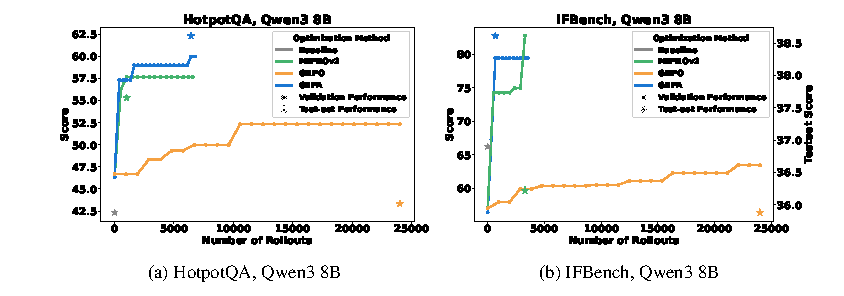
\includegraphics[width=\linewidth,height=0.68\textheight,keepaspectratio]{figure/gepa/fig_obs1_grpo_rollouts}
      \par\vspace{0.2em}{\color{Muted}\scriptsize Biểu đồ Score theo Rollout Budget --- GEPA (ICLR 2026)}
    \end{column}
  \end{columns}
\end{frame}

% ------------------------------------------------------------------ 37
\begin{frame}{2.4\quad Kết quả thực nghiệm}
  \Sub{Observation 2: Vượt trội MIPROv2 trên cả mô hình Mở \& Đóng}
  \begin{columns}[T,onlytextwidth]
    \begin{column}{0.44\textwidth}
      \begin{itemize}\setlength{\itemsep}{0.55em}
        \item GEPA vượt \textbf{MIPROv2} trên tất cả benchmark ở cả \textbf{Qwen3 8B}
              lẫn \textbf{GPT-4.1 mini} (trung bình cao hơn $>10\%$)
        \item Chứng minh \textbf{Đột biến Phản chiếu $+$ Biên Pareto} hiệu quả hơn hẳn
              tìm kiếm tổ hợp Bayesian dựa trên điểm số tổng
        \item Hiệu quả ổn định ngay cả khi không thể cập nhật trọng số mô hình (API đóng)
      \end{itemize}
    \end{column}
    \begin{column}{0.53\textwidth}
      \centering
      % FIGURE PLACEHOLDER (chua co file): figure/gepa/fig_obs2_main_table
      % \includegraphics[width=\linewidth,height=0.68\textheight,keepaspectratio]{figure/gepa/fig_obs2_main_table}
      \par\vspace{0.2em}{\color{Muted}\scriptsize Bảng/Biểu đồ so sánh tổng thể --- GEPA (ICLR 2026)}
    \end{column}
  \end{columns}
\end{frame}

% ------------------------------------------------------------------ 38
\begin{frame}{2.4\quad Kết quả thực nghiệm}
  \Sub{Observation 3: Prompt ngắn gọn hơn $\rightarrow$ Tiết kiệm Inference Token Budget}
  \begin{columns}[T,onlytextwidth]
    \begin{column}{0.46\textwidth}
      \begin{itemize}\setlength{\itemsep}{0.55em}
        \item \textbf{MIPROv2} có xu hướng nhồi nhiều ví dụ \textit{few-shot} để kéo điểm
              $\rightarrow$ prompt rất dài
        \item \textbf{GEPA} tổng hợp lỗi sai thành các \textbf{quy tắc cô đọng}
              $\rightarrow$ độ dài prompt ngắn hơn tới \textbf{$9\times$} so với MIPROv2
        \item Giúp giảm mạnh \textbf{chi phí suy luận (Inference Token Budget)} và độ trễ
              khi triển khai thực tế
      \end{itemize}
    \end{column}
    \begin{column}{0.51\textwidth}
      \centering
      % FIGURE PLACEHOLDER (chua co file): figure/gepa/fig_obs3_prompt_length
      % \includegraphics[width=\linewidth,height=0.68\textheight,keepaspectratio]{figure/gepa/fig_obs3_prompt_length}
      \par\vspace{0.2em}{\color{Muted}\scriptsize So sánh độ dài Prompt / Chi phí suy luận --- GEPA (ICLR 2026)}
    \end{column}
  \end{columns}
\end{frame}

% ------------------------------------------------------------------ 39
\begin{frame}{2.4\quad Kết quả thực nghiệm}
  \Sub{Observation 4: Tác động của Biên Pareto \& System-aware Merge}
  \begin{columns}[T,onlytextwidth]
    \begin{column}{0.46\textwidth}
      \begin{itemize}\setlength{\itemsep}{0.55em}
        \item \textbf{Biên Pareto vs. Tham lam (Greedy):} Chọn lọc Pareto luôn cho điểm
              cao và ổn định hơn nhờ giữ đa dạng chiến lược, tránh kẹt cực trị địa phương
        \item \textbf{System-aware Merge (LCA):}
          \begin{itemize}\tightlist
            \item Trên mô hình mạnh (\textbf{GPT-4.1 mini}): \texttt{GEPA+Merge} giúp cộng
                  thêm $\sim$5\% điểm so với \texttt{GEPA} thường.
            \item Trên mô hình nhỏ (\textbf{Qwen3 8B}): nhạy cảm với thời điểm ghép; ghép
                  quá sớm đôi khi làm điểm trung bình hơi giảm.
          \end{itemize}
      \end{itemize}
    \end{column}
    \begin{column}{0.51\textwidth}
      \centering
      % FIGURE PLACEHOLDER (chua co file): figure/gepa/fig_obs4_ablation
      % \includegraphics[width=\linewidth,height=0.68\textheight,keepaspectratio]{figure/gepa/fig_obs4_ablation}
      \par\vspace{0.2em}{\color{Muted}\scriptsize Kết quả Ablation (Pareto / Merge) --- GEPA (ICLR 2026)}
    \end{column}
  \end{columns}
\end{frame}

%=======================================================================
%  Slides 40-41 - 2.5 Giới hạn & Tổng kết
%=======================================================================

% ------------------------------------------------------------------ 40
\begin{frame}{2.5\quad Giới hạn \& Tổng kết}
  \Sub{Giới hạn của GEPA}
  \begin{itemize}\setlength{\itemsep}{0.6em}
    \item \textbf{Phụ thuộc vào Reflection LM \& chất lượng phản hồi ($\mu_f$):}\\
          Cần một LLM đủ mạnh để chẩn đoán đúng nguyên nhân gốc rễ; hiệu quả sẽ giảm nếu
          bài toán chỉ có điểm số thô mà không có dấu vết thực thi (traces) hoặc phản hồi
          lỗi rõ ràng.
    \item \textbf{Độ nhạy của System-aware Merge:}\\
          Hiệu quả ghép nhánh phụ thuộc vào năng lực mô hình và thời điểm kích hoạt (tăng
          mạnh trên GPT-4.1 mini nhưng dễ làm tụt nhẹ điểm trên mô hình nhỏ như Qwen3 8B
          nếu ghép quá sớm).
    \item \textbf{Giới hạn trần của việc đóng băng trọng số ($\theta$):}\\
          Chỉ tối ưu trên không gian văn bản nên khó giải quyết các tác vụ đòi hỏi nạp tri
          thức chuyên ngành hoàn toàn mới hoặc vượt quá năng lực suy luận sẵn có của mô hình
          gốc.
  \end{itemize}
\end{frame}

% ------------------------------------------------------------------ 41
\begin{frame}{2.5\quad Giới hạn \& Tổng kết}
  \Sub{Tổng kết (Key Takeaways)}
  \begin{itemize}\setlength{\itemsep}{0.55em}
    \item \textbf{Phản hồi ngôn ngữ $>$ Điểm thưởng vô hướng:} Khai thác Execution Traces
          qua Đột biến Phản chiếu giúp vượt trội RL (GRPO) với số lượt Rollout ít hơn tới
          \textbf{$35\times$}.
    \item \textbf{Tiến hóa cho hệ thống đa module:} Kết hợp \textbf{Biên Pareto} (giữ đa
          dạng chiến lược, chống overfit) và \textbf{System-aware Merge (LCA)} giúp tối ưu
          hiệu quả Compound AI System.
    \item \textbf{Tối ưu chi phí triển khai:} Sinh ra prompt ngắn gọn (ngắn hơn tới
          \textbf{$9\times$} so với MIPROv2), giảm mạnh \textit{Inference Token Budget} và
          áp dụng được cho cả API mô hình đóng.
  \end{itemize}
  \vspace{0.35em}
  \begin{beamercolorbox}[wd=\linewidth,sep=0.55em]{block body}
    \textbf{Mở rộng:} Khi tối ưu Prompt chạm trần do trọng số bị đóng băng $\rightarrow$
    cần chuyển sang hướng thích nghi tham số hiệu quả (\textbf{PEFT / Text-to-LoRA}).
  \end{beamercolorbox}
\end{frame}
%=======================================================================
%  Section 3 - PEFT: Text-to-LoRA (ICML 2025)
%   3.1 Bài toán   3.2 Liên quan   3.3 T2L (Module 1-4)   3.4 Thực nghiệm
%=======================================================================
\section{PEFT: Text-to-LoRA}

% ------------------------------------------------------------------ 3.1
\begin{frame}{3.1\quad Bài toán}{Khi có một tác vụ mới cần mô hình làm tốt}
  \Ask{Bạn sẽ làm gì? Fine-tune LoRA cho tác vụ mới --- và nếu đã có sẵn một số tác vụ rất giống thì sao?}

  \vspace{0.4em}
  \begin{columns}[T,onlytextwidth]
    \begin{column}{0.32\textwidth}
      \begin{beamercolorbox}[wd=\linewidth,sep=0.45em]{block body}
        \footnotesize\textbf{Nén các LoRA cũ bằng SVD}\\[0.15em]
        {\scriptsize\color{Muted}Tiết kiệm bộ nhớ, nhưng hiệu năng giảm.}
      \end{beamercolorbox}
    \end{column}
    \begin{column}{0.32\textwidth}
      \begin{beamercolorbox}[wd=\linewidth,sep=0.45em]{block body}
        \footnotesize\textbf{Chọn $k$ LoRA gần nhất}\\[0.15em]
        {\scriptsize\color{Muted}Bị giới hạn bởi các tác vụ cũ đã có.}
      \end{beamercolorbox}
    \end{column}
    \begin{column}{0.32\textwidth}
      \begin{beamercolorbox}[wd=\linewidth,sep=0.45em]{block alert body=AmberSoft,block alerted title}%
        \footnotesize\textbf{Dùng hypernetwork sinh adapter}\\[0.15em]
        {\scriptsize\color{Muted}Nhưng HN cũ nhận task-ID hoặc câu hỏi mẫu: bị giới hạn bởi tác vụ cũ, tốn train, và người dùng \emph{không kiểm soát} được.}
      \end{beamercolorbox}
    \end{column}
  \end{columns}

  \Takeaway{Mong muốn: \emph{một mô hình có thể sinh adapter từ chính mô tả của người dùng} --- không cần dữ liệu nhãn, không cần train lại.}
\end{frame}

% ------------------------------------------------------------------ 3.2
\begin{frame}{3.2\quad Công trình liên quan}{Hypernetwork}
  \begin{columns}[T,onlytextwidth]
    \begin{column}{0.47\textwidth}
      \justifying
      \textbf{Hypernetwork} là một mạng \emph{sinh ra trọng số} cho một mạng khác
      $W_l = h_\theta(\phi_l)$, với $\phi_l$ là mô tả của layer $l$
      (one-hot hoặc vector học được).

      \vspace{0.4em}
      Ý tưởng áp vào PEFT: thay vì sinh cả $W$ ($N\times N$), sinh các
      \emph{ma trận adapter} LoRA hạng thấp $\Delta W = BA$.
    \end{column}
    \begin{column}{0.47\textwidth}
      \centering
      \begin{tikzpicture}[font=\scriptsize, node distance=0.22cm,
          b/.style={draw=Navy, fill=Panel, rounded corners=2pt, minimum height=0.8cm, text width=2.5cm, align=center}]
        \node[b] (phi) {descriptor $\phi_l$};
        \node[b, fill=Navy, text=white, below=of phi] (h) {hypernetwork $h_\theta$};
        \node[b, below=of h] (w) {$W_l$ ($N\times N$)};
        \draw[-{Stealth}] (phi)--(h); \draw[-{Stealth}] (h)--(w);
        \node[right=0.15cm of w, text=Red!60!black, font=\tiny, text width=1.5cm, align=left] {quá lớn: $N^2$};
      \end{tikzpicture}\\[0.5em]
      \begin{tikzpicture}[font=\scriptsize, node distance=0.22cm,
          b/.style={draw=Navy, fill=Panel, rounded corners=2pt, minimum height=0.8cm, text width=2.5cm, align=center}]
        \node[b] (z) {mô tả tác vụ $z$};
        \node[b, fill=Navy, text=white, below=of z] (h2) {hypernetwork $h_\theta$};
        \node[b, below=of h2] (ab) {$A\in\mathbb{R}^{r\times d}$, $B\in\mathbb{R}^{d\times r}$};
        \draw[-{Stealth}] (z)--(h2); \draw[-{Stealth}] (h2)--(ab);
        \node[right=0.15cm of ab, text=PaperGreen, font=\tiny, text width=1.5cm, align=left] {nhỏ: $2rd$};
      \end{tikzpicture}
    \end{column}
  \end{columns}
  \Takeaway{Bước chuyển chính: đầu vào hypernetwork từ \emph{ID / câu hỏi mẫu} sang \emph{văn bản mô tả} --- thứ người dùng viết được.}
\end{frame}

% ------------------------------------------------------------------ 3.3
\begin{frame}{3.3\quad Text-to-LoRA}{Một mô hình sinh adapter từ mô tả}
  \begin{columns}[T,onlytextwidth]
    \begin{column}{0.46\textwidth}
      \justifying\footnotesize
      Khi có một tác vụ mới, T2L dùng \textbf{mô tả tác vụ} (trong paper do
      GPT-4o-mini sinh) làm đầu vào cho hypernetwork, từ đó sinh ra các ma trận
      adapter cho mô hình ngôn ngữ.

      \vspace{0.5em}
      \begin{beamercolorbox}[wd=\linewidth,sep=0.5em]{block body}
        \footnotesize
        \textbf{Một lượt chạy xuôi} $\rightarrow$ một bộ LoRA hoàn chỉnh.
        Không gradient, không dữ liệu nhãn, không chờ train.
      \end{beamercolorbox}
    \end{column}
    \begin{column}{0.5\textwidth}
      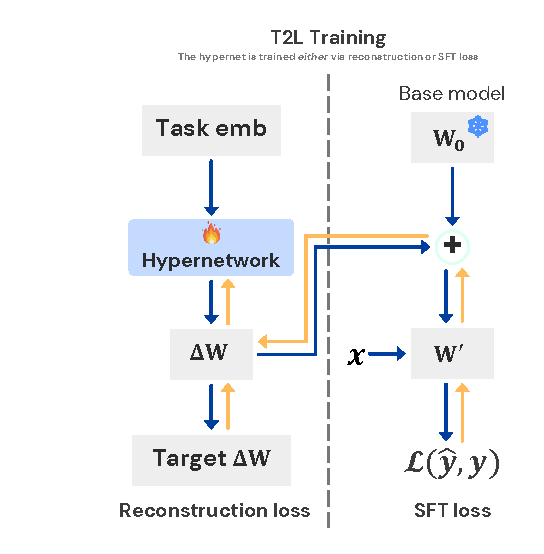
\includegraphics[width=\linewidth,height=0.47\textheight,keepaspectratio]{figure/t2l/fig1_train}%
      \par\vspace{0.2em}{\color{Muted}\scriptsize Fig 1 (trái): huấn luyện T2L --- tối ưu bằng reconstruction hoặc SFT.}
    \end{column}
  \end{columns}
\end{frame}

\begin{frame}{3.3\quad Module 1 --- Kiến trúc}{Architecture L / M / S}
  \FigureFull[0.42]{t2l/fig2_arch}{Fig 2: biến thể kiến trúc của T2L. Hộp xanh là module trainable, hộp cyan là embedding trainable; $r$ là hạng LoRA, $d$ là chiều ẩn.}
  \begin{columns}[T,onlytextwidth]
    \begin{column}{0.63\textwidth}
      \small
      \[
        \Delta W_{m,l}=h_\theta\!\left(\operatorname{concat}\big[f(z),\,E[m],\,E[l]\big]\right)
      \]
      \footnotesize\justifying
      $z$: mô tả tác vụ, $f$: text encoder, $E[m]$: loại module (key/value),
      $E[l]$: chỉ số layer.
    \end{column}
    \begin{column}{0.33\textwidth}
      \footnotesize
      Thêm $E[m]$ và $E[l]$ làm đầu vào là để \emph{một} bộ trọng số hypernetwork
      sinh được adapter cho mọi layer, mọi module.
    \end{column}
  \end{columns}
\end{frame}

\begin{frame}{3.3\quad Module 1 --- Cùng lúc sinh nhiều cặp (A,B)}
  \begin{columns}[T,onlytextwidth]
    \begin{column}{0.48\textwidth}
      \textbf{Vấn đề:} lớp FC đầu ra của hypernetwork sẽ khổng lồ nếu sinh cả $W$
      ($N\times N$). Chuyển sang một cặp $(A,B)$ kiểu LoRA đã nhỏ hơn nhiều ---
      nhưng Mistral-7B có 32 layer transformer $\Rightarrow$ cần một bộ adapter cho
      mỗi layer và mỗi module.

      \vspace{0.4em}
      Với hidden cuối $=512$, sinh đủ cho 7B bằng một lần sẽ cần
      $\approx 1.7$ tỉ tham số đầu ra.
    \end{column}
    \begin{column}{0.48\textwidth}
      \textbf{Cách của T2L:} thêm hai thuộc tính làm input ---
      \emph{layer thứ mấy} và \emph{module key hay value} --- rồi
      \textbf{chạy hypernetwork theo batch} cho mọi $(m,l)$ cùng lúc.

      \vspace{0.4em}
      Vì một lượt chạy chỉ mất vài chục mili giây, chạy 64 lần cho 64 cặp $(A,B)$
      vẫn nhanh hơn nhiều so với train LoRA.
    \end{column}
  \end{columns}
  \vspace{0.5em}
  \Takeaway{Chi phí tham số giảm từ $\sim$1.7B xuống $\sim$55M, còn thời gian vẫn tính bằng phần trăm giây.}
\end{frame}

\begin{frame}{3.3\quad Module 1 --- Ba mức đầu ra: L, M, S}
  \begin{columns}[T,onlytextwidth]
    \begin{column}{0.56\textwidth}
      \noindent\resizebox{\linewidth}{!}{%
      \small
      \setlength{\tabcolsep}{5pt}
      \begin{tabular}{@{}l l l c r@{}}
        \toprule
        Biến thể & Đầu ra & Input thêm & Batch & Tham số \\
        \midrule
        \textbf{L} & cả $A$ và $B$ & --- & 64 & $\sim$55M \\
        \textbf{M} & $A$ \emph{hoặc} $B$ & A/B emb & 128 & $\sim$34M \\
        \textbf{S} & một \emph{hàng} của $A$/$B$ & A/B $+$ rank emb & 1024 & $\sim$5M \\
        \bottomrule
      \end{tabular}}\\[0.4em]
      {\scriptsize\color{Muted}Ba biến thể đổi output kích thước lớn thành nhiều lần chạy nhỏ.}
    \end{column}
    \begin{column}{0.4\textwidth}
      \centering
      \begin{tikzpicture}[font=\scriptsize]
        \foreach \i/\n/\p/\c in {1/S/5/15, 2/M/34/45, 3/L/55/75}{%
          \pgfmathsetmacro{\bh}{\p/12}
          \fill[Navy!\c] (\i-0.38,0) rectangle (\i+0.38,\bh);
          \node[above, font=\scriptsize] at (\i,\bh) {\textbf{\n}};
          \node[below, font=\scriptsize, text=Muted] at (\i,0) {\p M};
        }
        \draw[Muted] (0.4,0) -- (3.6,0);
        \node[font=\scriptsize, text=Muted] at (2,2.1) {tham số đầu ra};
      \end{tikzpicture}
    \end{column}
  \end{columns}
  \Takeaway{Không phải chọn một: paper cho thấy cả ba đều cạnh tranh, và S nhẹ nhất lại mạnh nhất trên một số tác vụ (PIQA).}
\end{frame}

\begin{frame}{3.3\quad Module 2 --- Độ nhạy với mô tả}{Cùng một bài toán, ba mô tả}
  \begin{columns}[T,onlytextwidth]
    \begin{column}{0.5\textwidth}
      {\footnotesize\color{Muted}Toulouse has twice as many sheep as Charleston. Charleston has 4 times as many sheep as Seattle. How many sheep do Toulouse, Charleston, and Seattle have together if Seattle has 20 sheep?}

      \vspace{0.25em}
      \begin{itemize}\tightlist\footnotesize
        \item \textbf{(i)} Mô hình gốc: giải đúng từng bước, CoT dài;
        \item \textbf{(ii)} Mô tả chất lượng kém \emph{“solve this task please”}:
              vẫn ra 240, nhưng rất ngắn;
        \item \textbf{(iii)} Mô tả thiên toán học: suy luận trực tiếp hơn, nhưng
              \emph{tính sai} ($260$);
        \item \textbf{(iv)} Mô tả thiên lập trình: tiếp cận thuật toán từng bước.
      \end{itemize}
    \end{column}
    \begin{column}{0.47\textwidth}
      \FigureFull[0.62]{t2l/fig4_qualitative}{Fig 4: cùng một câu hỏi, LoRA sinh từ bốn mô tả khác nhau cho bốn phong cách trả lời khác nhau.}
    \end{column}
  \end{columns}
  \Takeaway{LoRA sinh ra \emph{steerable}: đổi mô tả là đổi hành vi --- nhưng vẫn có thể sai (như ví dụ iii).}
\end{frame}

\begin{frame}{3.3\quad Module 3 --- Text encoder}{Tại sao dùng encoder ngoài, và tại sao là gte-large-en}
  \begin{columns}[T,onlytextwidth]
    \begin{column}{0.48\textwidth}
      \begin{beamercolorbox}[wd=\linewidth,sep=0.55em]{block title}
        \centering Tại sao không dùng encoder của LM?
      \end{beamercolorbox}
      \vspace{0.3em}
      \footnotesize\justifying
      Encoder của LM đã được huấn luyện cho \emph{mục tiêu khác} (dự đoán token).
      Paper dẫn lập luận của HINT và HyperTune: một text encoder \emph{độc lập},
      chuyên cho biểu diễn câu, cho embedding mô tả tốt hơn --- và giữ LM không
      phải sửa.
    \end{column}
    \begin{column}{0.48\textwidth}
      \begin{beamercolorbox}[wd=\linewidth,sep=0.55em]{block title}
        \centering Vì sao là gte-large-en-v1.5?
      \end{beamercolorbox}
      \vspace{0.3em}
      \footnotesize\justifying
      Tại thời điểm viết paper (2025), đây là một trong những encoder nhỏ mạnh nhất
      ở nhiệm vụ embedding câu, chỉ $\sim$400M tham số --- đủ nhẹ để chạy cạnh
      hypernetwork.

      \vspace{0.3em}
      T2L dùng activation của token CLS ở layer cuối (model là bidirectional).
    \end{column}
  \end{columns}
  \vspace{0.4em}
  \Takeaway{Đọc kỹ: encoder \emph{không} phải thứ được train trong SFT --- hypernetwork mới là thứ học.}
\end{frame}

\begin{frame}{3.3\quad Module 4 --- Hai cách train hypernetwork}
  \begin{columns}[T,onlytextwidth]
    \begin{column}{0.48\textwidth}
      \begin{beamercolorbox}[wd=\linewidth,sep=0.55em]{block title}
        \centering Reconstruction
      \end{beamercolorbox}
      \vspace{0.3em}
      \footnotesize\justifying
      \begin{enumerate}\tightlist
        \item Train sẵn LoRA riêng cho \emph{từng} tác vụ trong thư viện;
        \item Hypernetwork sinh adapter, so với adapter thật bằng MSE;
        \item Cập nhật hypernetwork.
      \end{enumerate}
      {\scriptsize\color{Muted}Cần trước một thư viện LoRA đã train.}
    \end{column}
    \begin{column}{0.48\textwidth}
      \begin{beamercolorbox}[wd=\linewidth,sep=0.55em]{block title}
        \centering SFT
      \end{beamercolorbox}
      \vspace{0.3em}
      \footnotesize\justifying
      \begin{enumerate}\tightlist
        \item Hypernetwork sinh adapter;
        \item Gắn adapter vào LM \emph{đóng băng} để trả lời câu hỏi;
        \item Dùng cross-entropy của câu trả lời để cập nhật hypernetwork.
      \end{enumerate}
      {\scriptsize\color{Muted}Học end-to-end trên tác vụ thật.}
    \end{column}
  \end{columns}
  \vspace{0.4em}
  \Takeaway{Reconstruction học “chép” trọng số; SFT học “làm đúng việc” --- và paper cho thấy khác biệt lớn.}
\end{frame}

\begin{frame}{3.3\quad Module 4 --- Reconstruction vs SFT}
  \begin{columns}[T,onlytextwidth]
    \begin{column}{0.5\textwidth}
      \centering\footnotesize
      \begin{tabular}{@{}lccc c@{}}
        \toprule
        & \multicolumn{3}{c}{Benchmark} & \\
        \cmidrule(lr){2-4}
        & S & M & L & TB \\
        \midrule
        Reconstruction & 61.8 & 61.7 & 62.0 & 61.8 \\
        \textbf{SFT}   & 64.8 & 66.5 & \Win{67.5} & \Win{66.3} \\
        \bottomrule
      \end{tabular}\\[0.5em]
      {\scriptsize\color{Muted}Bảng 6: cùng khoảng thời gian train ($\sim$10 giờ) cho mỗi cấu hình.}
    \end{column}
    \begin{column}{0.46\textwidth}
      \textbf{Tại sao SFT thắng?}
      \begin{itemize}\tightlist\footnotesize
        \item Hai bộ trọng số khác nhau có thể cho cùng hành vi
              $\Rightarrow$ \emph{không đồng nhất nghiệm tối ưu} của MSE;
        \item MSE đo khoảng cách trọng số, \emph{không} đo độ tốt của mô hình;
        \item SFT bỏ được yêu cầu thư viện LoRA: học trực tiếp từ mục tiêu cuối.
      \end{itemize}
    \end{column}
  \end{columns}
  \vspace{0.3em}
  \Takeaway{Đây là lập luận cốt lõi của paper: mục tiêu cuối là \emph{trả lời đúng}, nên loss phải đo điều đó.}
\end{frame}

% ------------------------------------------------------------------ 3.4
\begin{frame}{3.4\quad Thực nghiệm}{So với task-specific LoRA (9 tác vụ đã thấy khi train)}
  \begin{columns}[T,onlytextwidth]
    \begin{column}{0.66\textwidth}
      \centering
      \resizebox{\linewidth}{!}{%
      \scriptsize
      \begin{tabular}{@{}l ccccccccc c@{}}
        \toprule
        & ArcC & ArcE & BQ & GSM8K & HS & OQA & PIQA & WG & MBPP & TB \\
        \midrule
        Base model              & 65.4 & 77.8 & 71.6 & 40.9 & 49.7 & 54.2 & 72.8 & 45.0 & 43.1 & 55.8 \\
        \midrule
        \multicolumn{11}{@{}l}{\scriptsize\color{Muted}One-hot task embedding} \\
        T2L (Recon) L           & \Win{76.4} & 89.9 & 89.4 & \Win{53.8} & 92.6 & 85.0 & 69.7 & 51.2 & 52.6 & \Win{73.4} \\
        T2L (Recon) M           & \Win{76.7} & 89.9 & 89.4 & 53.2 & 92.6 & 85.0 & 69.9 & 51.4 & 52.9 & \Win{73.4} \\
        T2L (Recon) S           & 75.2 & 88.8 & 87.4 & 50.9 & 89.1 & 75.6 & \Win{83.9} & \Win{58.1} & 48.1 & 73.0 \\
        \midrule
        \multicolumn{11}{@{}l}{\scriptsize\color{Muted}Task description embedding} \\
        T2L (Recon) L           & 76.6 & 89.8 & 89.4 & 53.9 & 92.6 & 85.0 & 69.6 & 51.2 & 51.8 & 73.3 \\
        T2L (Recon) M           & 76.5 & 89.9 & 89.4 & 53.9 & 92.5 & 84.9 & 70.4 & 51.6 & 52.8 & \Win{73.5} \\
        T2L (Recon) S           & 75.4 & 88.8 & 87.8 & 49.1 & 89.7 & 76.7 & \Win{84.2} & \Win{56.9} & 48.0 & 73.0 \\
        \midrule
        Task-specific LoRA (oracle) & 76.6 & 89.9 & 89.4 & 53.5 & 92.6 & 85.0 & 69.9 & 51.1 & 52.1 & 73.3 \\
        \bottomrule
      \end{tabular}}
    \end{column}
    \begin{column}{0.3\textwidth}
      \footnotesize\justifying
      T2L \textbf{khôi phục gần như hoàn toàn} hiệu năng LoRA oracle, và
      \textbf{vượt oracle} ở nhiều tác vụ.

      \vspace{0.4em}
      Lý do được paper đưa ra: nén \emph{lossy} đóng vai trò như
      regularization --- rõ nhất ở PIQA và WG, nơi oracle LoRA bị overfit.
    \end{column}
  \end{columns}
\end{frame}

\begin{frame}{3.4\quad Thực nghiệm}{Zero-shot trên tác vụ \emph{chưa} thấy khi train}
  \begin{columns}[T,onlytextwidth]
    \begin{column}{0.6\textwidth}
      \centering
      \resizebox{\linewidth}{!}{%
      \scriptsize
      \begin{tabular}{@{}l cccccccc c cc c@{}}
        \toprule
        & ArcC & ArcE & BQ & HS & OQA & PIQA & WG & MBPP & TB(8) & GSM8K & HE & TB(10) \\
        \midrule
        No test-time adaptation \\
        \quad Mistral-7B-Instruct & 65.4 & 77.8 & 71.6 & 49.7 & 54.2 & 72.8 & 45.0 & 43.1 & 60.0 & 40.9 & 37.2 & 55.8 \\
        \quad Prepending task desc. & 72.0 & 85.8 & 67.6 & 58.9 & 63.4 & 77.9 & 59.0 & 41.6 & 65.8 & 40.9 & 39.0 & 60.6 \\
        \quad 3-shot ICL & 72.1 & 85.9 & 71.7 & 59.0 & 66.2 & 76.2 & 58.0 & 42.6 & 66.5 & 40.9 & 37.2 & 61.0 \\
        \quad Multi-task LoRA & 76.2 & 88.3 & \Win{85.5} & 65.2 & 68.0 & 81.8 & 62.4 & 48.1 & 71.9 & 47.5 & 39.6 & 66.3 \\
        \midrule
        Zero-shot adaptation \\
        \quad Arrow Routing & 60.9 & 86.2 & 87.6 & 80.8 & 48.6 & 83.0 & 68.5 & \Win{50.2} & 70.7 & --- & 28.7 & --- \\
        \quad Hyperdecoders & \Win{76.6} & 88.5 & 83.9 & 65.2 & \Win{76.6} & 81.3 & 64.9 & 51.6 & \Win{73.6} & 43.6 & \Win{40.9} & 67.3 \\
        \quad T2L (SFT) S & 76.0 & 88.7 & 83.8 & \Win{68.0} & 71.6 & \Win{82.3} & 61.0 & 41.2 & 71.6 & \Win{47.3} & 39.0 & 65.9 \\
        \quad T2L (SFT) M & 77.2 & 89.0 & 84.3 & 65.1 & 76.1 & 81.8 & 64.0 & 50.5 & 73.5 & 45.2 & \Win{41.3} & 67.5 \\
        \quad \textbf{T2L (SFT) L} & \Win{77.5} & \Win{88.9} & 85.0 & 66.5 & 75.5 & 82.1 & 64.2 & 51.9 & \Win{73.9} & 45.8 & 39.2 & \Win{67.7} \\
        \bottomrule
      \end{tabular}}
    \end{column}
    \begin{column}{0.36\textwidth}
      \begin{itemize}\tightlist\footnotesize
        \item T2L \textbf{vượt multi-task LoRA} một cách nhất quán;
        \item Vượt cả oracle ở một số tác vụ;
        \item Chưa đóng hết khoảng cách với LoRA riêng từng tác vụ;
        \item Arrow Routing không sinh được adapter cho tác vụ quá xa.
      \end{itemize}
      \vspace{0.3em}
      {\scriptsize\color{Muted}Bảng 2 (rút gọn): TB(8) bỏ GSM8K và HumanEval, TB(10) gồm cả hai.}
    \end{column}
  \end{columns}
\end{frame}

\begin{frame}{3.4\quad Thực nghiệm}{T2L mở rộng tốt khi có nhiều tác vụ train hơn}
  \begin{columns}[T,onlytextwidth]
    \begin{column}{0.44\textwidth}
      \FigureFull[0.6]{t2l/fig1_scaling}{Fig 1 (phải): điểm zero-shot trên 10 benchmark khi tăng số tập dữ liệu pretrain.}
    \end{column}
    \begin{column}{0.5\textwidth}
      \begin{itemize}\tightlist\footnotesize
        \item Từ 64 lên 479 tác vụ, cả L/M/S đều tăng điểm;
        \item Trên 479 tác vụ: L đạt \textbf{67.7}, M 67.5, S 65.2;
        \item T2L vượt \textbf{MT-LoRA} --- baseline fine-tune multi-task thường;
        \item Nhưng vẫn sau oracle LoRA riêng cho từng tác vụ.
      \end{itemize}
      \vspace{0.3em}
      \FigureFull[0.26]{t2l/fig3_error}{Fig 3: điểm tương đối so với oracle giảm khi lỗi reconstruction tăng --- nén là \emph{lossy}.}
    \end{column}
  \end{columns}
\end{frame}

%=======================================================================
%  Slide 55 - Chi phí và hạn chế  (1:1 with slide-cs222.pptx.pdf)
%=======================================================================
\section{Chi phí \& Hạn chế}

\begin{frame}{Chi phí và hạn chế}
  \vspace{1.2em}
  \centering
  \begin{tikzpicture}[font=\normalsize,
      card/.style={fill=white, draw=Rule, rounded corners=5pt, minimum height=3.4cm,
                   anchor=north west, inner sep=0.35cm}]
    % card 1
    \node[card, fill=AmberSoft, draw=Amber, text width=3.2cm, align=left] (c1) at (0,0) {%
      {\scriptsize\color{Muted} T2L: sinh LoRA + trả lời}\\[0.4em]
      {\color{Amber!85!black}\fontsize{30}{32}\selectfont\bfseries 0,86}\\[0.3em]
      {\small TFLOPs mỗi câu}};
    % card 2
    \node[card, text width=3.2cm, align=left, right=0.35cm of c1.north east, anchor=north west] (c2) {%
      {\scriptsize\color{Muted} 3-shot ICL}\\[0.4em]
      {\color{Navy}\fontsize{30}{32}\selectfont\bfseries 4,18}\\[0.3em]
      {\small TFLOPs mỗi câu}};
    % card 3
    \node[card, fill=Panel, text width=5.0cm, align=left, right=0.35cm of c2.north east, anchor=north west] (c3) {%
      {\bfseries\color{Navy} Hạn chế}\\[0.5em]
      {\small Phụ thuộc chất lượng mô tả (trong paper do GPT-4o-mini viết)}\\[0.5em]
      {\small Chưa thử chuyển từ model nhỏ sang model lớn}};
  \end{tikzpicture}
\end{frame}

%=======================================================================
%  The source deck ends at slide 55 (Chi phí và hạn chế); it has no
%  reference or summary slides, so none are added here.
%=======================================================================


\end{document}
